%
% File acl2014.tex
%
% Contact: giovanni.colavizza@epfl.ch
%%
%% Based on the style files for ACL-2013, which were, in turn,
%% Based on the style files for ACL-2012, which were, in turn,
%% based on the style files for ACL-2011, which were, in turn, 
%% based on the style files for ACL-2010, which were, in turn, 
%% based on the style files for ACL-IJCNLP-2009, which were, in turn,
%% based on the style files for EACL-2009 and IJCNLP-2008...

%% Based on the style files for EACL 2006 by 
%%e.agirre@ehu.es or Sergi.Balari@uab.es
%% and that of ACL 08 by Joakim Nivre and Noah Smith

\documentclass[11pt]{article}
\usepackage{acl2014}
\usepackage{times}
\usepackage{url}
\usepackage{latexsym}
 \usepackage{todonotes}
 \usepackage{float}
 \usepackage{listings}
 
\usepackage[colorlinks]{hyperref}
\hypersetup{citecolor=DeepPink4}
\hypersetup{linkcolor=DarkRed}
\hypersetup{urlcolor=DarkBlue}
\usepackage{cleveref}

%\setlength\titlebox{5cm}

% You can expand the titlebox if you need extra space
% to show all the authors. Please do not make the titlebox
% smaller than 5cm (the original size); we will check this
% in the camera-ready version and ask you to change it back.


\title{An ecological study of the food industry}

\author{Veillard Jennifer \\
  {\tt jennifer.veillard@epfl.ch} \\\And
  \\\textbf{Lanzrein Johan} \\
  {\tt johan.lanzrein@epfl.ch} \\\And
Freundler Nicolas \\
{\tt nicolas.freundler@epfl.ch} \\}

\date{}

\begin{document}
\maketitle
\begin{abstract}
As ecology grows as a more important concern, populations need not only to focus on driving less or consuming less, but also on how they consume food. It is a known fact that consuming products derived from palm oil, or meat in general is much more damaging for the environment than growing your own vegetables. During this project, we aim to expose how to be more regarding towards the environment in our daily food consumption.
The main goal is to investigate the world of food and understand what are some hints to take when we want to consume more eco-friendly.
\end{abstract}

\section{Introduction}

We decided to focus on the main ecological issues related with our daily food consumption. We first start to look into our dataset and notice how it is distributed and from this biased distribution we have to adjust our analysis. Afterwards, we compute the distance related information. We explore different aspect that are related to ecology, such as palm oil, vegan products, and labeling.  
A solution often presented is to eat locally. Thus we were interested in knowing what are the distance typically travelled by a product from its origin or manufacturing place until its selling place.
Finally, we explore how Switzerland relates to its neighboring countries when it comes to labels.


\section{Dataset Description}
This project used the Open Food Facts database. This database compiles information about food around the world in an collaborative way. This means any user can add information about a food product she/he has to improve the database. In our study, we focus on mainly the following informations : 
\begin{itemize}
    \item Labels (vegan, green dot,...) described as $labels\_en$
    \vspace{-0.3cm}
    \item Palm oil information under fields such as $ingredients\_from\_palm\_oil\_n$
    \vspace{-0.3cm}
    \item Distance travelled from $origins\_tags$ or $manufacturing\_ places\_tags$ to $countries\_en$
    %\item Country where it is sold 
    %\item Category of product the column is $categories\_en$
\end{itemize}

\noindent
For each of those, we will make a link with the category of the product (column $categories\_en$).

\section{Pre-processing}
During the preprocessing phase, we create different datasets that each contain the relevant information to answer a specific problem. %about an item. 
%Moreover, we create a dataset containing the distance each item has travelled by using the origin and country fields. \\
At this point, we notice how the dataset is flawed. As it is a collaborative dataset anyone can enter information and often we get fields that are empty which will clearly be detrimental for the analysis. To counter this we take a few measures. First of all, we decide to focus the study on France, as the database contains much more product from France then anywhere else. 
\vspace{-0.3cm}

\begin{figure}[h]
\centering
\includegraphics[width=.95\linewidth]{figures/countries_withFrance.png}
\label{fig:fig1a}
\caption{Number product sold in each country (top 15 countries)}
\label{fig:fig1}
\end{figure}

\noindent
In the end we have the following csv files that can be used throughout the project : 

%\vspace{-0.5cm}

\begin{itemize}
    \item \textit{DistancePerProduct}: computed for each product with selling country and an origin or a manufacturing place specified. Basically the distance between both places is computed using the geopy library.
    \vspace{-0.3cm}
    \item \textit{FrenchProduct}: all products sold in France.
    \vspace{-0.3cm}
    \item \textit{labels} : all products with a labels
    \vspace{-0.3cm}
    \item \textit{vegan} : all products which label is vegan
    \vspace{-0.3cm}
    \item \textit{palm\_oil} : all products with information about palm oil
\end{itemize}

\noindent
In addition, the csv file \textit{SeveralNamesOneCountry} contains a dataset used to build a dictionary to translate the countries names. Briefly, not all the nouns in \textit{countries\_en} are in English, this dictionary will give the English correspondence.

%\todo[inline, color = blue!40]{On devrait être plus clair de dire où ont été utilisé toutes les données et où c'est seulement celles de la France}

\section{Data exploration}
As a start, we compute how many articles we have total in the data set. 
We found a total of 665693 articles entered. 
\subsection{Palm oil}
As palm oil is known for being a major factor for deforestation, we wanted to study what kind of products contain the most palm oil. We select items that contain palm oil and then look for the biggest category (see figure~\ref{fig:cat_palm_oil}). As expected, categories such as cookies and snacks contain a lot of palm oil products.
\begin{figure}
    \centering
    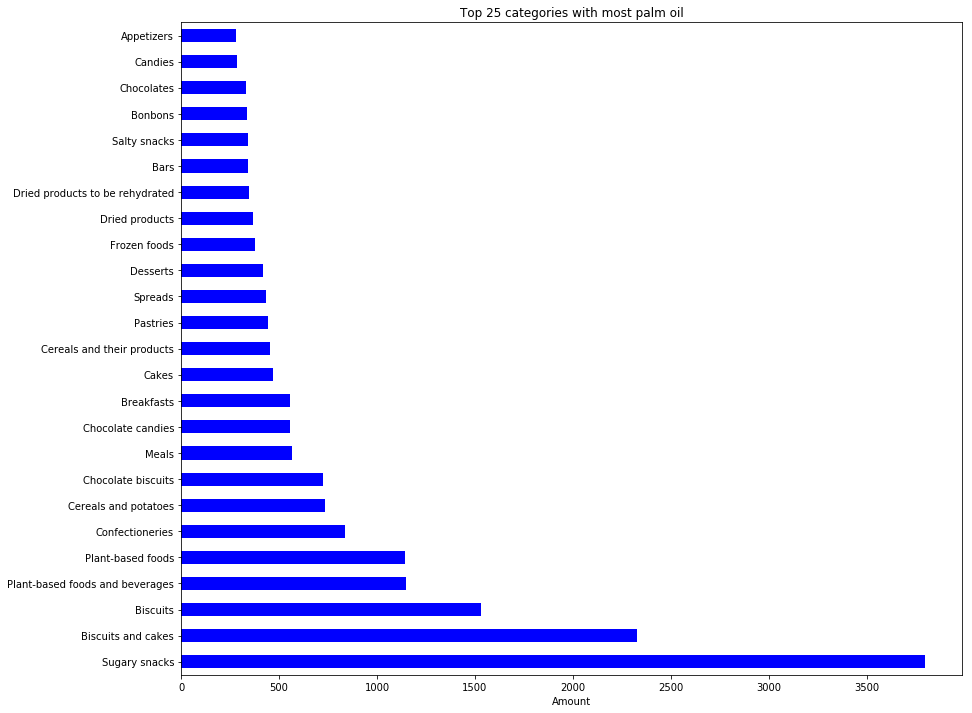
\includegraphics[scale=0.2]{figures/top_categories_palm_oil.png}
    \caption{Categories consuming the most palm oil}
    \label{fig:cat_palm_oil}
\end{figure}
\noindent
Moreover we also look at the evolution of number of palm oil articles over time. We notice that the number of articles containing palm oil follows a quadratic trend. So we could infer that there is more articles over time.
\subsubsection{Labels and palm oil}
When a consumer wants to avoid palm oil, he has no choice but to try and decipher the ingredients list. However there might be some indicators such as the label that could strongly suggest that the product contains palm oil. We explore this and found that there exists in fact an organization called RSPO (Roundtable on Sustainable Palm Oil ), which delivers labels that can be found on products. The most prominent labels can be found on the figure ~\ref{fig:normal_lab_palm_oil}. 

\vspace{-0.3cm}
\begin{figure}[H]
    \centering
    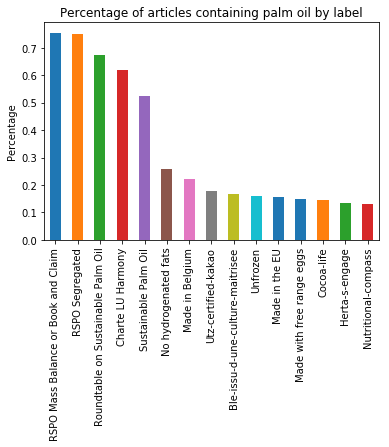
\includegraphics[scale=0.4]{figures/palm_oil_labels_normalized_2.png}
    \caption{Percentage of articles containing palm oil by label}
    \label{fig:normal_lab_palm_oil}
\end{figure}


\subsection{Labels}
We found that labels concerning ecological and organic food products were the most popular however they represent only a fraction of the total dataset. There are a variety of labels. We decided to focus on two main labels that are related to sustainable food consummation. The first ones are labels that are related to ecological food preparation. Secondly, we investigate vegan product. Veganism has been argued to be an eco-friendly as it produces less waste and uses less ressources. 
\subsubsection{Ecological labels}
Investigating labels related to ecological products, we found that : 
\begin{itemize}
    \item There are 37395 articles with label organic. This represents 0.056175 \% of articles 
    \item There are 13886 articles with label bio
This represents 0.020859 \% of articles 
\end{itemize}

After our analysis, we saw that the most present labels were for instance Organic, Green Dot, and EU Organic. Hence even though there is a minority of products that are certified Organic, they are still the most present label in our dataset.

\subsubsection{Vegan}



Although the debate is still ongoing about sustainability of cutting dairies and meats from diet, people tend to adopt a vegan life-style, because of their anti-
speciesism ideology or their will to reduce carbon footprint of their diet. For more information about this subject on link : \href{https://www.independent.co.uk/life-style/health-and-families/veganism-environmental-impact-planet-reduced-plant-based-diet-humans-study-a8378631.html}{The Independent}.

In our data base, some products were labelled 'vegan' and were compared with the remaining data. One has to be careful that some product are labelled 'non-vegan' and too simple regex operation can take them as false-positives.

A first glance at origin distribution during preprocessing indicates that most of vegan-labelled products of our data base comes from France but Spain.


\subsection{Distance relationships}
Eating locally is an eco-friendly alternative. To understand clearly what kind of product travel a lot until reaching the supermarket we were interested in computing the distance. Answering this question was less straight-forward then the previous ones. A preprocessing set has to be done to select the data containing both a starting point (either origin or manufacturing place) and an arrival point (country, where the product is sold). In both cases, those data were transformed into coordinate thanks to geopy and then the distance computation was done using the same library. 

In figure ~\ref{fig:network_france}, we can see that products consummed by the french market are mainly from france, with Spain and Italy being behind. 
\vspace{-0.3cm}
\begin{figure}[H]
    \centering
    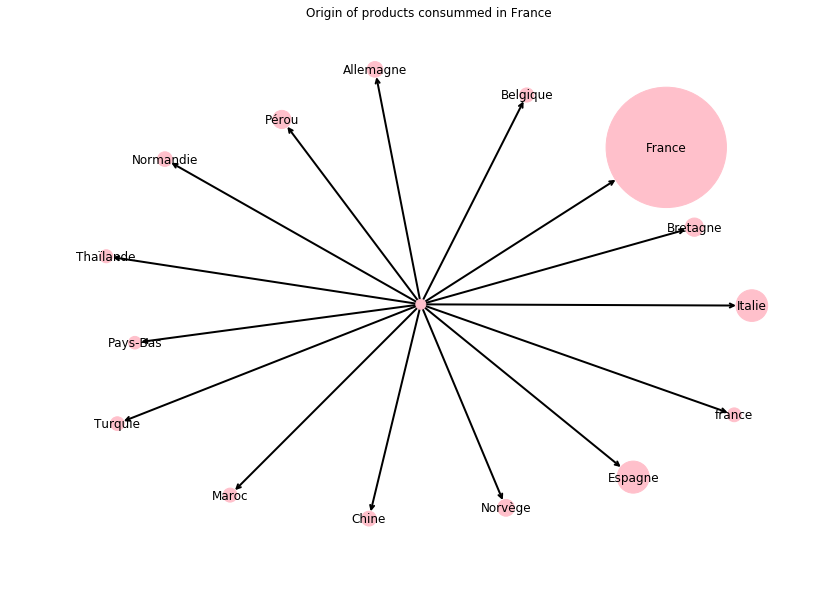
\includegraphics[scale=0.25]{figures/origin_food_france_network.png}
    \caption{Network graph displaying origins of food products}
    \label{fig:network_france}
\end{figure}


\subsubsection{Category and distance}
In this section, we investigate which are the kind of product that travel more than others. We also focus only on french products. 
The hypothesis is that some category of products such as dairies and maybe meats will travel less than prepared meals for instance. 
To do this, we use the computations done beforehand and apply them to products before grouping them by category to see if we find any relations. We notice for instance that  
As can be seen in the figure ~\ref{fig:dairies_fruit}, the distribution varies depending on the products. We noticed a major peak at the [0,2500] and the [7500,10000] bins. The distance from France to for example South America is in the bracket of 7500km and 10000km so we can suppose that exotic products such as cocoa beans for chocolate come from this area. 

\vspace{-0.3cm}
\begin{figure}[H]
    \centering
    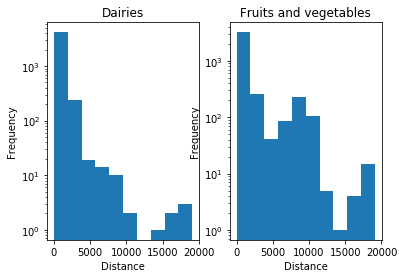
\includegraphics[scale=0.4]{figures/compare_dairies_fruits_distance.png}
    \caption{Comparison between dairies and fruits related products by distance}
    \label{fig:dairies_fruit}
\end{figure}



% \subsection{Relationship between label and distance}

% Eating locally and eating organic are both presented as more suitable solution, we wanted to look if those product are correlated. Meaning are organic product produced closer to the selling place. %Our logic would tell that both have to be correlated but who did not face the question in a supermarket : do I take those local tomatoes or that ones that are organic but come from Spain ?

%\todo{if its relevant relationship between label -- distance}

\section{Statistical analysis}
\subsection{Distribution comparison}

Distribution of fat and sugar was done between vegan-labelled and other products. The standard ones are paired-t tests, but they only apply to normally distributed population with same variances.

There exist a non-parametric paired-test for non-normal distributions based on ranks, called Wilcoxon test.

The histogram of fat and energy distributions on both classes strongly suggest non-normality of those features, as shown on \ref{fig:histo_comp}. The Wilcoxon test was then performed. The hypotheses "Same distribution" and "Vegan more caloric" were rejected with p-values of respectively  9.60e-13 4.80e-13. Finally, the hypothesis "Vegan is less caloric" was not rejected with a p-value of 1.00.

The results for fat distribution are similar but a bit less stringer: for equivalent hypotheses for fat, the p-values are respectively 4.52e-5, 2.26e-5 and 1.00.

The equivalence between these two features is not surprising given that Spearman's correlation between energy and fat is 0.79 in vegan food and 0.74 in non-vegan data (p-values both 0.0).
https://www.overleaf.com/1184642841swhbqhvmcvmx
\vspace{-0.3cm}
\begin{figure}[H]
    \centering
    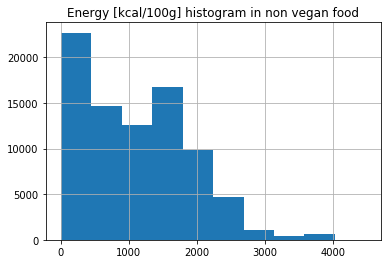
\includegraphics[scale=0.37]{figures/non_vegan_energy.png}
    \caption{Energy distribution of non-vegan and vegan food}
    \label{fig:histo_comp}
\end{figure}

%\subsection{Correlations}

\subsection{Association rule learning}
Association rules are usually used in market basket analysis. The concept is to compute probabilities for a customer to purchase some items given that he/she has already purchase other ones.
We adapted this method with two different features: the eco-friendly  labels (Organic, EU Organic, Green Point) and the different categories (beverages, meals, ...). For instance, the association rule "  EU Organic $\rightarrow$ Beverages " is equivalent to compute P(Category= Beverages $|$ Label = EU Organic).

It is important to take in account only relevant local rules. To compute the relevance of rules "A $\rightarrow$ B" and "B $\rightarrow$ A", one computes the joined probability P(category = A, label = EU Organic). The twenty highest supports on the whole data set were kept for designing association rules.

Rules were computed for the total data set, for France and its neighbors. They were used a mean to compare eco-label consumption in those different countries.

As it can be tedious to compare association rules one by one, they were taken as a 1D vector. The similarity between two vectors can be computed with cosine similarity or linear correlation. As there is not any theoretical reason to prefer one method to an other one. We also adapted Tanimoto's distance that is normally used for bit strings, in order to test if it can be used for small real number vector comparison.
%\begin{equation}
%    LinCorrelation=\frac{\sum{(x_i-\bar{x})(y_i-\bar{y})}}{\sqrt{\sum{(x_i-\bar{x})^2}\sum{(y_i-\bar{y})^2}}}
%\end{equation}
%\begin{equation}
%    CosineSimilarity=\frac{\sum{x_i y_i}}{\sqrt{\sum{x_i^2}\sum{y_i^2}}}
%\end{equation}
%\vspace{-1cm}
\begin{equation}
    Tanimoto=\frac{\sum{x_i y_i}}{\sum{x_i^2}+\sum{y_i^2}-\sum{x_i y_i}}
\end{equation}

%\vspace{-1cm}
The results show that the similarity assessment are not equivalent on our data: if country A is more similar to B in cosine similarity than to C, it is not necessarily true according Tanimoto's and linear correlation similarities. Belgium and France are more similar than Belgium and the rest of the world with linear correlation (0.76 vs 0.75) and cosine (0.55 vs 0.53) similarity, but it is the opposite with Tanimoto's (0.57 vs 0.58).
In general France, Italy, Germany and the total data set have higher similarities measurements.


To visualize the results, the association vector were projected onto a 2D subspace. The immediate draw back of such a method is that dimensionality reduction might be too high and ignore some important information. Dimensionality was performed with three different techniques: principle componant analysis (PCA), independant componant analysis (ICA) and a autoencoder neural network (NN). For any of the techniques, data are normalized before execution.

%\begin{itemize}
     

%     \item PCA projects the data onto a space were the new features are uncorrelated. PCA reduces dimensionality by taking the principal components with highest variances. Principal components are linearly uncorrelated.
%     \item ICA: coming from signal source demixing problem, ICA tries to retrieve the weights of the different sources, under the assumption that the pure sources are non gaussian.
%     \item The autoencoder NN is  has different hidden layers, including the coder which has a low number of neurons. The NN is trained to reproduced the same data from input to output. Once trained 300 times, values at the coder layer represent a non-linear projection of data onto a lower dimensional space.
%\end{itemize}   

Besides different scales of latent features, the three method show similar results, there are central clouds formed by Italy, Germany, France and World (the total data), whereas Spain, Belgium and Switzerland are outsiders, as shown in \ref{fig:PCA}.
\begin{figure}[H]
    \centering
    \includegraphics[scale=0.36]{figures/datavizir.png}
    \caption{Dimensionality reduction of association rules by PCA and by autoencoder with 2x 128-neuron layers, 2x 64-neuron layers 1x 2-neuron layer and 300 epochs}
    \label{fig:PCA}
\end{figure}


 

\section{Conclusion}
Throughout this analysis of the Open Food Facts Database, we first noticed how incomplete real world datasets can be. This added the challenge of working with the incompleteness of the set. We learned how to complete information with external library such as geopy. Moreover we applied general data analysis technique seen during class to observe trends in the data. In the end, we used machine learning techniques to learn whether some European countries had similar behaviors. \\
The study of ecology in food is a subject that will be even more important in the future years. As society advances and the number of humans continues to augment, we need to look into sustainable and ecological way to produce food such that every human can have access to products. 

% \section{General Instructions}

% Manuscripts must be in two-column format.  Exceptions to the
% two-column format include the title, authors' names and complete
% addresses, which must be centered at the top of the first page, and
% any full-width figures or tables (see the guidelines in
% Subsection~\ref{ssec:first}). {\bf Type single-spaced.}  Start all
% pages directly under the top margin. See the guidelines later
% regarding formatting the first page.

% \subsection{Format of Electronic Manuscript}
% \label{sect:pdf}

% For the production of the electronic manuscript you must use Adobe's
% Portable Document Format (PDF). PDF files are usually produced from
% \LaTeX\ using the \textit{pdflatex} command. If your version of
% \LaTeX\ produces Postscript files, you can convert these into PDF
% using \textit{ps2pdf} or \textit{dvipdf}. On Windows, you can also use
% Adobe Distiller to generate PDF.

% Please make sure that your PDF file includes all the necessary fonts
% (especially tree diagrams, symbols, and fonts with Asian
% characters). When you print or create the PDF file, there is usually
% an option in your printer setup to include none, all or just
% non-standard fonts.  Please make sure that you select the option of
% including ALL the fonts. \textbf{Before sending it, test your PDF by
%   printing it from a computer different from the one where it was
%   created.} Moreover, some word processors may generate very large PDF
% files, where each page is rendered as an image. Such images may
% reproduce poorly. In this case, try alternative ways to obtain the
% PDF. One way on some systems is to install a driver for a postscript
% printer, send your document to the printer specifying ``Output to a
% file'', then convert the file to PDF.

% It is of utmost importance to specify the \textbf{A4 format} (21 cm
% x 29.7 cm) when formatting the report. When working with
% {\tt dvips}, for instance, one should specify {\tt -t a4}.

% Print-outs of the PDF file on A4 report should be identical to the
% hardcopy version.


% \subsection{Layout}
% \label{ssec:layout}

% Format manuscripts two columns to a page, in the manner these
% instructions are formatted. The exact dimensions for a page on A4
% report are:

% \begin{itemize}
% \item Left and right margins: 2.5 cm
% \item Top margin: 2.5 cm
% \item Bottom margin: 2.5 cm
% \item Column width: 7.7 cm
% \item Column height: 24.7 cm
% \item Gap between columns: 0.6 cm
% \end{itemize}

% \noindent Papers should not be submitted on any other report size, no exceptions.


% \subsection{Fonts}

% For reasons of uniformity, Adobe's {\bf Times Roman} font should be
% used. In \LaTeX2e{} this is accomplished by putting

% \begin{quote}
% \begin{verbatim}
% \usepackage{times}
% \usepackage{latexsym}
% \end{verbatim}
% \end{quote}
% in the preamble. If Times Roman is unavailable, use {\bf Computer
%   Modern Roman} (\LaTeX2e{}'s default).  Note that the latter is about
%   10\% less dense than Adobe's Times Roman font.


% \begin{table}[h]
% \begin{center}
% \begin{tabular}{|l|rl|}
% \hline \bf Type of Text & \bf Font Size & \bf Style \\ \hline
% report title & 15 pt & bold \\
% author names & 12 pt & bold \\
% the word ``Abstract'' & 12 pt & bold \\
% section titles & 12 pt & bold \\
% document text & 11 pt  &\\
% captions & 11 pt & \\
% abstract text & 10 pt & \\
% bibliography & 10 pt & \\
% footnotes & 9 pt & \\
% \hline
% \end{tabular}
% \end{center}
% \caption{\label{font-table} Font guide.}
% \end{table}

% \subsection{The First Page}
% \label{ssec:first}

% Center the title and author's name(s) across both
% columns. Do not use footnotes for affiliations. Use the
% two-column format only when you begin the abstract.

% {\bf Title}: Place the title centered at the top of the first page, in
% a 15-point bold font. (For a complete guide to font sizes and styles,
% see Table~\ref{font-table}) Long titles should be typed on two lines
% without a blank line intervening. Approximately, put the title at 2.5
% cm from the top of the page, followed by a blank line, then the
% author's names(s) on the following line. Do not
% use only initials for given names (middle initials are allowed). Do
% not format surnames in all capitals (e.g., use ``Schlangen'' not
% ``SCHLANGEN'').  Do not format title and section headings in all
% capitals as well except for proper names (such as ``BLEU'') that are
% conventionally in all capitals. Start the body of the first page 7.5 cm from the top of the
% page.

% {\bf Abstract}: Type the abstract at the beginning of the first
% column. The width of the abstract text should be smaller than the
% width of the columns for the text in the body of the report by about
% 0.6 cm on each side. Center the word {\bf Abstract} in a 12 point bold
% font above the body of the abstract. The abstract should be a concise
% summary of the general thesis and conclusions of the report. It should
% be no longer than 150 words. The abstract text should be in 10 point font.

% {\bf Text}: Begin typing the main body of the text immediately after
% the abstract, observing the two-column format as shown in 
% the present document. Do not include page numbers.

% {\bf Indent} when starting a new paragraph. Use 11 points for text and 
% subsection headings, 12 points for section headings and 15 points for
% the title. 

% \subsection{Sections}

% {\bf Headings}: Type and label section and subsection headings in the
% style shown on the present document.  Use numbered sections (Arabic
% numerals) in order to facilitate cross references. Number subsections
% with the section number and the subsection number separated by a dot,
% in Arabic numerals. Do not number subsubsections.

% {\bf Citations}: Citations within the text appear in parentheses
% as~\cite{Gusfield:97} or, if the author's name appears in the text
% itself, as Gusfield~\shortcite{Gusfield:97}.  Append lowercase letters
% to the year in cases of ambiguity.  Treat double authors as
% in~\cite{Aho:72}, but write as in~\cite{Chandra:81} when more than two
% authors are involved. Collapse multiple citations as
% in~\cite{Gusfield:97,Aho:72}. Also refrain from using full citations
% as sentence constituents. We suggest that instead of
% \begin{quote}
%   ``\cite{Gusfield:97} showed that ...''
% \end{quote}
% you use
% \begin{quote}
% ``Gusfield \shortcite{Gusfield:97}   showed that ...''
% \end{quote}

% If you are using the provided \LaTeX{} and Bib\TeX{} style files, you
% can use the command \verb|\newcite| to get ``author (year)'' citations.

% \textbf{Please do not use anonymous citations} and do not include
% acknowledgements when submitting your reports..

% \textbf{References}: Gather the full set of references together under
% the heading {\bf References}. Arrange the references alphabetically
% by first author, rather than by order of occurrence in the text.
% Provide as complete a citation as possible, using a consistent format,
% such as the one for {\em Computational Linguistics\/} or the one in the 
% {\em Publication Manual of the American 
% Psychological Association\/}~\cite{APA:83}.  Use of full names for
% authors rather than initials is preferred.  A list of abbreviations
% for common computer science journals can be found in the ACM 
% {\em Computing Reviews\/}~\cite{ACM:83}.

% \subsection{Footnotes}

% {\bf Footnotes}: Put footnotes at the bottom of the page and use 9
% points text. They may be numbered or referred to by asterisks or other
% symbols.\footnote{This is how a footnote should appear.} Footnotes
% should be separated from the text by a line.\footnote{Note the line
% separating the footnotes from the text.}

% \subsection{Graphics}

% {\bf Illustrations}: Place figures, tables, and photographs in the
% report near where they are first discussed, rather than at the end, if
% possible.  Wide illustrations may run across both columns.

% {\bf Captions}: Provide a caption for every illustration; number each one
% sequentially in the form:  ``Figure 1. Caption of the Figure.'' ``Table 1.
% Caption of the Table.''  Type the captions of the figures and 
% tables below the body, using 11 point text.

% \begin{thebibliography}{}

% \bibitem[\protect\citename{Aho and Ullman}1972]{Aho:72}
% Alfred~V. Aho and Jeffrey~D. Ullman.
% \newblock 1972.
% \newblock {\em The Theory of Parsing, Translation and Compiling}, volume~1.
% \newblock Prentice-{Hall}, Englewood Cliffs, NJ.

% \bibitem[\protect\citename{{American Psychological Association}}1983]{APA:83}
% {American Psychological Association}.
% \newblock 1983.
% \newblock {\em Publications Manual}.
% \newblock American Psychological Association, Washington, DC.

% \bibitem[\protect\citename{{Association for Computing Machinery}}1983]{ACM:83}
% {Association for Computing Machinery}.
% \newblock 1983.
% \newblock {\em Computing Reviews}, 24(11):503--512.

% \bibitem[\protect\citename{Chandra \bgroup et al.\egroup }1981]{Chandra:81}
% Ashok~K. Chandra, Dexter~C. Kozen, and Larry~J. Stockmeyer.
% \newblock 1981.
% \newblock Alternation.
% \newblock {\em Journal of the Association for Computing Machinery},
%   28(1):114--133.

% \bibitem[\protect\citename{Gusfield}1997]{Gusfield:97}
% Dan Gusfield.
% \newblock 1997.
% \newblock {\em Algorithms on Strings, Trees and Sequences}.
% \newblock Cambridge University Press, Cambridge, UK.

% \end{thebibliography}

\end{document}